Flow control defines how network resources are allocated when data is transmitted from a source node to a destination node through multiple routers and links. Its main purpose is to coordinate the use of communication channels and buffers, especially when multiple packets compete for the same network resource at the same time.

At a high level, two basic switching approaches can be considered: circuit switching and packet switching. In circuit switching, a complete communication path is established before data transmission begins, and the reserved path remains occupied until the transfer is finished. This approach can provide predictable transmission behavior once the connection is set up, but it suffers from long setup time and low channel utilization, since reserved resources may remain idle during parts of the transmission. For this reason, circuit switching is generally not suitable for scalable on-chip communication systems.

In contrast, packet switching does not require a dedicated end-to-end path to be reserved in advance. Instead, a message is divided into smaller transmission units and forwarded hop by hop through the network. This improves resource utilization and allows multiple messages to share the same physical channels. In NoC design, packet switching is more widely adopted because it provides better flexibility and higher throughput under dynamic traffic conditions.

In a packet-switched NoC, data is usually organized hierarchically as message, packet, and flit, as shown in Figure~\ref{fig:packet_flit}. A message is the complete unit of communication between two nodes. A message may be divided into one or more packets, and each packet may be further divided into several flits. The flit is the basic unit handled by the router for flow control. Based on how packets and flits are buffered and forwarded, several packet-switched flow control strategies have been proposed, including store-and-forward, virtual cut-through, and wormhole switching \cite{Danashtalab2014}. These strategies differ mainly in their buffer requirements, latency, and hardware complexity. Among them, wormhole switching is widely used in NoCs because it reduces buffer demand while maintaining relatively efficient packet forwarding. In wormhole switching, a packet is divided into flits, where the head flit carries routing information and establishes the path, the body flits follow the reserved path, and the tail flit releases the occupied resources after the transmission is completed.

\begin{figure}[htbp]
    \centering
    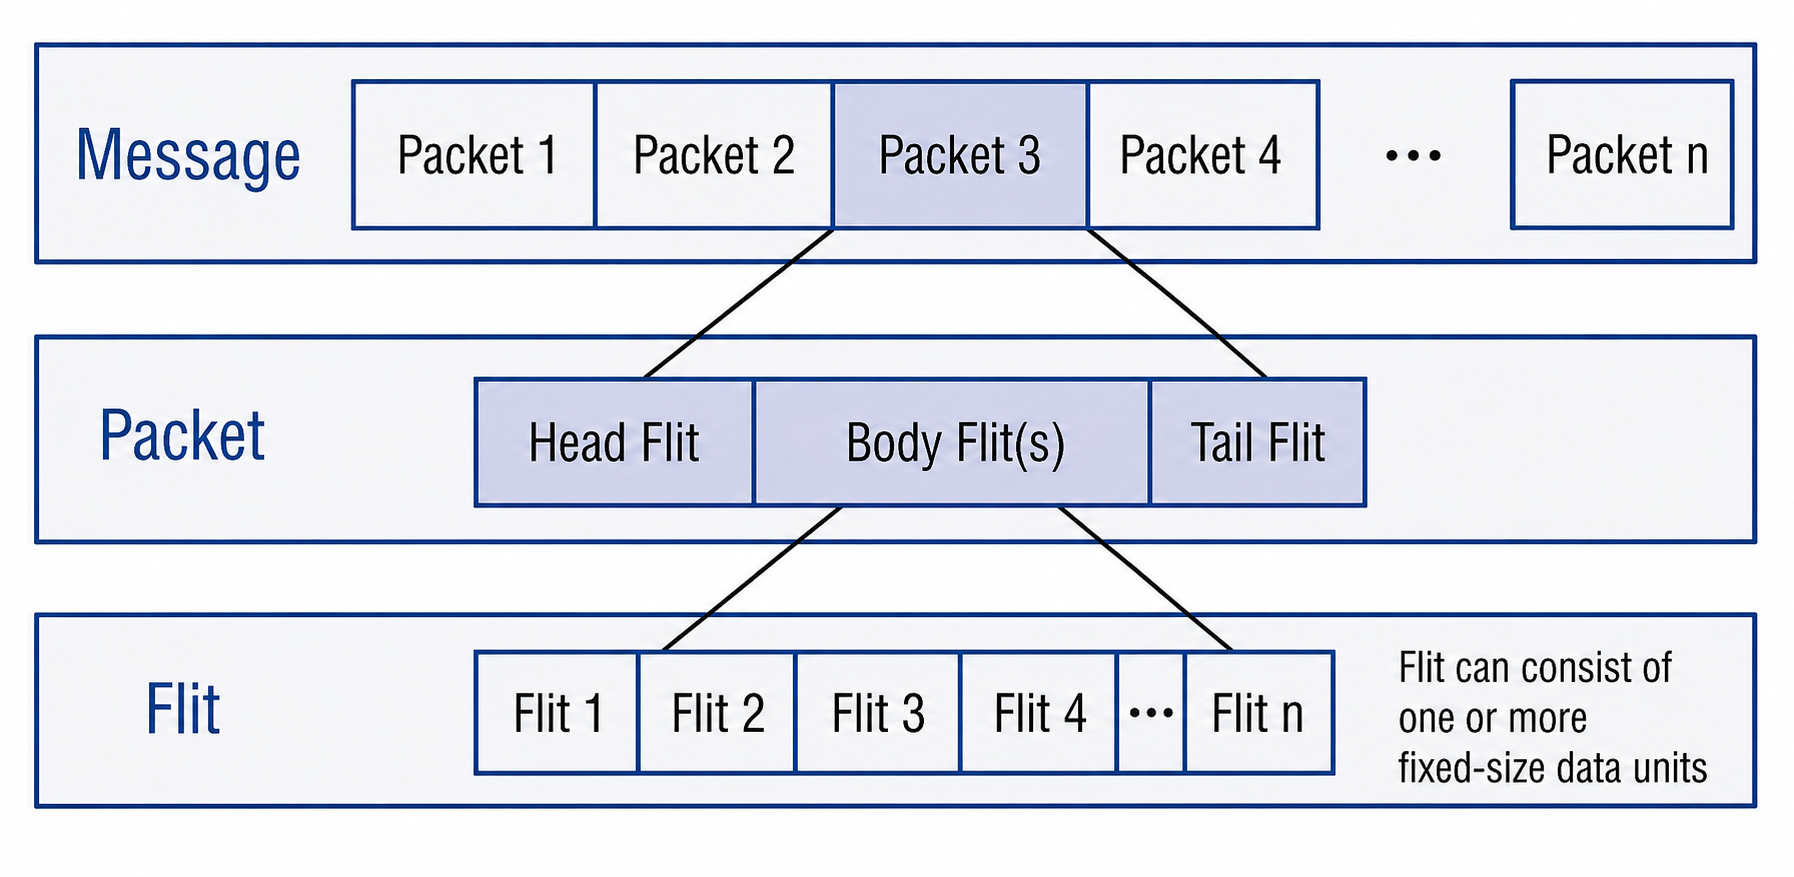
\includegraphics[width=0.8\textwidth]{images/ch2background/packet_flit.png}
    \caption{Packet and flit organization}
    \label{fig:packet_flit}
\end{figure}

Since this thesis focuses on routing and router design in a NoC-based communication structure, packet-switched flow control is adopted, and wormhole switching is used as the main data transmission mechanism.
